\section{Dipendenza della frequenza dalla tensione}

Successivamente è stata studiata la dipendenza della frequenza della seconda armonica dalla tensione applicata alla corda.
Mantenendo costante la lunghezza del tratto vibrante, sono state variate le masse appese al sistema di carrucola e supporto, modificando così la tensione della corda.
I dati misurate sono mostrati in Tabella 2.

\begin{table}[H]
\centering
\begin{tabular}{ccc}
\hline
\textbf{Massa appesa} \textbf{(\unit{\kilogram})} & \textbf{Frequenza} \textbf{(\unit{\hertz})} & \textbf{Incertezza} \textbf{(\unit{\hertz})} \\
\hline
0.08062 & 32.0 & 1.0 \\
0.09061 & 33.0 & 1.0 \\
0.11058 & 37.0 & 1.0 \\
0.13048 & 40.0 & 1.0 \\
0.15045 & 42.0 & 1.0 \\
0.18034 & 47.0 & 1.0 \\
0.28036 & 57.0 & 1.0 \\
0.38008 & 65.0 & 1.0 \\
\hline
\end{tabular}
\caption{Frequenze misurate al variare della tensione applicata alla corda.}
\end{table}

Si interpola linearmente la frequenza in funzione della radice quadrata della tensione, assumendo un'incertezza di $\sigma_f = \qty{1.0}{\hertz}$ sulle misure di frequenza, seguendo lo stesso criterio adottato per le misure effettuate nella precedente sezione dell'esperienza.

\begin{figure}[H]
    \centering
    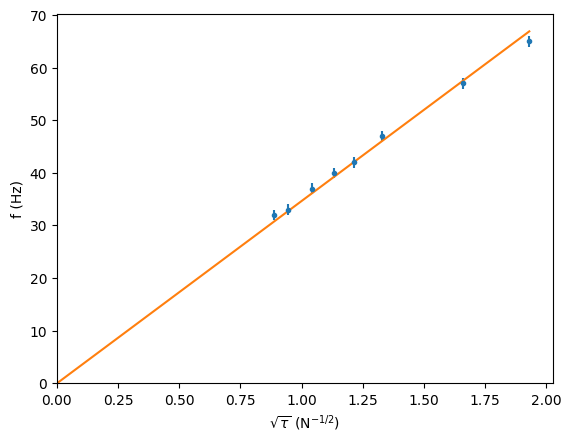
\includegraphics[width=0.6\textwidth]{Immagini/2.png}
    \caption{Interpolazione con un parametro libero della frequenza in funzione della radice quadrata della tensione applicata alla corda.}
\end{figure}

Il test del $\chi^2$ restituisce un $\Tilde{\chi}_o^2$=1.10, che per sette gradi di libertà corrisponde ad una probabilità del 36.2\%.
Il coefficiente angolare interpolato è $k_2 = \qty{34.65 \pm 0.27}{\hertz\newton\tothe{\text{-1/2}}}$, mentre quello ricavato dalla relazione \eqref{eq:frequenze} è $k'_2 = \qty{33.2 \pm 1.8}{\hertz\newton\tothe{\text{-1/2}}}$. \\
Tramite la relazione \eqref{eq:t_test} si ottiene $t_0 = 0.79$, che corrisponde a una probabilità di accordo tra le misure del 43.0\%.